% !TeX spellcheck = en_US
% !TeX root = tikz-ext-manual.tex
% Copyright 2022 by Qrrbrbirlbel
%
% This file may be distributed and/or modified
%
% 1. under the LaTeX Project Public License and/or
% 2. under the GNU Free Documentation License.
%

\section{Transformations: Mirroring}
\label{pgflibrary:transformations}

\begin{purepgflibrary}{ext.transformations.mirror}
  This library adds mirror transformations to \pgfname.
\end{purepgflibrary}

Two approaches to mirror transformation exist:
\begin{enumerate}
\item Using the reflection matrix (see left column).

  This depends on |\pgfpointnormalised|\indexCommandO\pgfpointnormalised which involves
  the sine\indexMathFunctionO{sin} and the cosine\indexMathFunctionO{cos} functions of \pgfname math.

\item Using built-in transformations (see right column).

  This depends on |\pgfmathanglebetweenpoints|\indexCommandO\pgfmathanglebetweenpoints which
  involves the arctangent (|atan2|\indexMathFunctionO{atan2}) function of \pgfname math.
\end{enumerate}

Which one is better? I don't know.
Choose one you're comfortable with.

\begin{paracol}{2}

\subsection{Using the reflection matrix}

The following commands use the reflection matrix that sets the transformation matrix following
\begin{equation*}
  A = \frac{1}{\Vert\vec l\Vert^2} \begin{bmatrix}
  l_x^2-l_y^2 & 2l_xl_y \\
  2l_xl_y & l_y^2-l_x^2\\
  \end{bmatrix}.
\end{equation*}

\switchcolumn% >

\stepcounter{subsection}
\subsection{Using built-in transformations}

The following commands use a combination of shifting, rotating, $-1$ scaling,
rotating back and shifting back to reach the mirror transformation.

The commands are named the same as on the left side,
only the |m| in |mirror| is capitalized.

\switchcolumn*% <

\begin{command}{\pgfexttransformxmirror\marg{value}}\cmdcompat\pgftransformxmirror
  Sets up a transformation that mirrors along a vertical line that goes through point $(\text{\meta{value}}, 0)$.

\begin{codeexample}[preamble=\usepgflibrary{ext.transformations.mirror}]
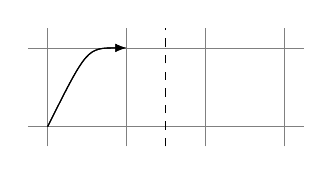
\begin{tikzpicture}
\draw[help lines] (-.25, -.25) grid (3.25, 1.25);
\draw[-latex] (0,0) .. controls (.5,1) .. (1,1);

\draw[dashed] (1.5, -.25) -- (1.5, 1.25);
\pgfexttransformxmirror{1.5}

\draw[-latex] (0,0) .. controls (.5,1) .. (1,1);
\end{tikzpicture}
\end{codeexample}
\end{command}

\switchcolumn% >

\begin{command}{\pgfexttransformxMirror\marg{value}}\cmdcompat\pgftransformxMirror
  Sets up a transformation that mirrors along a vertical line that goes through point $(\text{\meta{value}}, 0)$.

\begin{codeexample}[preamble=\usepgflibrary{ext.transformations.mirror}]
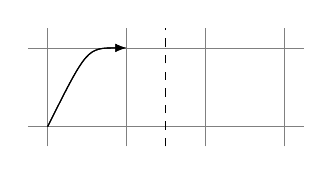
\begin{tikzpicture}
\draw[help lines] (-.25, -.25) grid (3.25, 1.25);
\draw[-latex] (0,0) .. controls (.5,1) .. (1,1);

\draw[dashed] (1.5, -.25) -- (1.5, 1.25);
\pgfexttransformxMirror{1.5}

\draw[-latex] (0,0) .. controls (.5,1) .. (1,1);
\end{tikzpicture}
\end{codeexample}
\end{command}

\switchcolumn*% <

\begin{command}{\pgfexttransformymirror\marg{value}}\cmdcompat\pgftransformymirror
  Sets up a transformation that mirrors along a horizontal line that goes through point $(0, \text{\meta{value})}$.
\end{command}

\begin{command}{\pgfexttransformmirror\marg{point A}\marg{point B}}\cmdcompat\pgftransformmirror
  Sets up a transformation that mirrors along the line that goes through \meta{point A} and \meta{point B}.
 
\begin{codeexample}[preamble=\usepgflibrary{ext.transformations.mirror}]
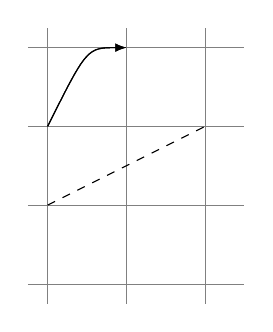
\begin{tikzpicture}
\draw[help lines] (-.25, -2.25) grid (2.5, 1.25);
\draw[-latex] (0,0) .. controls (.5,1) .. (1,1);

\draw[dashed] (0, -1) -- (2, 0);
\pgfexttransformmirror{\pgfpointxy{0}{-1}}
                      {\pgfpointxy{2}{ 0}}

\draw[-latex] (0,0) .. controls (.5,1) .. (1,1);
\end{tikzpicture}
\end{codeexample}
\end{command}

\switchcolumn% >

\begin{command}{\pgfexttransformyMirror\marg{value}}\cmdcompat\pgftransformyMirror
  Sets up a transformation that mirrors along a horizontal line that goes through point $(0, \text{\meta{value})}$.
\end{command}

\begin{command}{\pgfexttransformMirror\marg{point A}\marg{point B}}\cmdcompat\pgftransformMirror
  Sets up a transformation that mirrors along the line that goes through \meta{point A} and \meta{point B}.
 
\begin{codeexample}[preamble=\usepgflibrary{ext.transformations.mirror}]
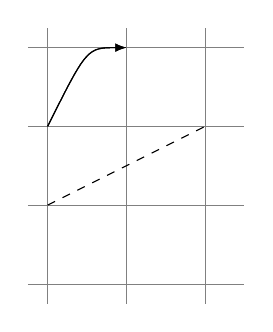
\begin{tikzpicture}
\draw[help lines] (-.25, -2.25) grid (2.5, 1.25);
\draw[-latex] (0,0) .. controls (.5,1) .. (1,1);

\draw[dashed] (0, -1) -- (2, 0);
\pgfexttransformMirror{\pgfpointxy{0}{-1}}
                      {\pgfpointxy{2}{ 0}}

\draw[-latex] (0,0) .. controls (.5,1) .. (1,1);
\end{tikzpicture}
\end{codeexample}
\end{command}

\switchcolumn*% <

\begin{command}{\pgfextqtransformmirror\marg{point A}}\cmdcompat\pgfqtransformmirror
  Sets up a transformation that mirrors along the line that goes through the origin and \meta{point A}.

\begin{codeexample}[preamble=\usepgflibrary{ext.transformations.mirror}]
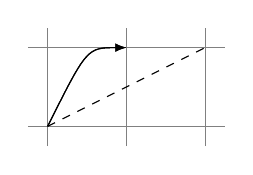
\begin{tikzpicture}
\draw[help lines] (-.25, -.25) grid (2.25, 1.25);
\draw[-latex] (0,0) .. controls (.5,1) .. (1,1);

\draw[dashed] (0, 0) -- (2, 1);
\pgfextqtransformmirror{\pgfpointxy{2}{1}}

\draw[-latex] (0,0) .. controls (.5,1) .. (1,1);
\end{tikzpicture}
\end{codeexample}
\end{command}

\switchcolumn

\begin{command}{\pgfextqtransformMirror\marg{point A}}\cmdcompat\pgfqtransformMirror
  Sets up a transformation that mirrors along the line that goes through the origin and \meta{point A}.

\begin{codeexample}[preamble=\usepgflibrary{ext.transformations.mirror}]
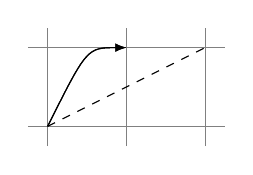
\begin{tikzpicture}
\draw[help lines] (-.25, -.25) grid (2.25, 1.25);
\draw[-latex] (0,0) .. controls (.5,1) .. (1,1);

\draw[dashed] (0, 0) -- (2, 1);
\pgfextqtransformMirror{\pgfpointxy{2}{1}}

\draw[-latex] (0,0) .. controls (.5,1) .. (1,1);
\end{tikzpicture}
\end{codeexample}
\end{command}

\end{paracol}
\endinput
